\documentclass[10pt,twocolumn,letterpaper]{article}
% Layout modelled on the REVTeX 4.2 two-column preprint style (Palatino text, centred small-caps
% section heads, "FIG." captions), built with standard packages.
\usepackage[T1]{fontenc}
\usepackage[sc]{mathpazo}
\linespread{1.04}
\usepackage[letterpaper,top=0.85in,bottom=0.9in,left=0.72in,right=0.72in,columnsep=0.28in]{geometry}
\usepackage{amsmath,amssymb}
\usepackage{graphicx}
\usepackage{booktabs}
\usepackage{xcolor}
\usepackage{microtype}
\usepackage{titlesec}
\usepackage{fancyhdr}
\usepackage[labelsep=colon,font=small,justification=justified,singlelinecheck=true]{caption}
\usepackage[sort&compress,numbers]{natbib}
\usepackage[colorlinks=true,linkcolor=blue!55!black,citecolor=blue!55!black,urlcolor=blue!55!black]{hyperref}
\usepackage{url}
\usepackage{orcidlink}
\usepackage{enumitem}
\usepackage{placeins}
\renewcommand{\topfraction}{0.9}\renewcommand{\bottomfraction}{0.8}\renewcommand{\textfraction}{0.07}\renewcommand{\floatpagefraction}{0.75}\renewcommand{\dbltopfraction}{0.9}\renewcommand{\dblfloatpagefraction}{0.75}
\setlist{nosep,leftmargin=1.2em}

% generated by make_numbers.py from report/stats.json and paper/paper_stats.json -- do not edit
\newcommand{\Version}{0.1.0}
\newcommand{\DOI}{10.5281/zenodo.24206837}
\newcommand{\NCounties}{3{,}144}
\newcommand{\NMetro}{1{,}164}
\newcommand{\NRural}{1{,}563}
\newcommand{\NFrontier}{417}
\newcommand{\NMetroFrontier}{22}
\newcommand{\NRF}{1{,}980}
\newcommand{\NBG}{239{,}741}
\newcommand{\NBGZero}{3{,}759}
\newcommand{\Women}{65{,}970{,}543}
\newcommand{\WomenMillions}{66.0}
\newcommand{\WomenRF}{8{,}047{,}307}
\newcommand{\WomenRFShare}{12.2}
\newcommand{\WomenFrontier}{423{,}145}
\newcommand{\WomenRural}{7{,}624{,}162}
\newcommand{\WomenMetro}{57{,}923{,}236}
\newcommand{\Vertices}{24.4}
\newcommand{\Arcs}{56.0}
\newcommand{\KmRoad}{8.0}
\newcommand{\KmFerry}{15{,}240}
\newcommand{\Components}{65{,}673}
\newcommand{\MainNetworks}{71}
\newcommand{\ShareMain}{99.17}
\newcommand{\BGNoRoad}{62}
\newcommand{\WomenNoRoad}{5{,}104}
\newcommand{\BGSep}{259}
\newcommand{\WomenSep}{2{,}083}
\newcommand{\SnapMedianM}{74}
\newcommand{\SnapPNinetyM}{343}
\newcommand{\SnapPNinetyNineKm}{1.05}
\newcommand{\SitesOB}{2{,}424}
\newcommand{\RoutedOB}{2{,}424}
\newcommand{\SitesOBU}{3{,}087}
\newcommand{\RoutedOBU}{3{,}087}
\newcommand{\SitesOBC}{9{,}343}
\newcommand{\RoutedOBC}{9{,}051}
\newcommand{\SitesPPW}{4{,}600}
\newcommand{\RoutedPPW}{4{,}584}
\newcommand{\SitesMH}{12{,}637}
\newcommand{\RoutedMH}{12{,}591}
\newcommand{\SitesHC}{11{,}769}
\newcommand{\RoutedHC}{11{,}706}
\newcommand{\SitesOBAdded}{663}
\newcommand{\AddedCAH}{599}
\newcommand{\AddedAcute}{64}
\newcommand{\CMSConfSM}{2{,}289}
\newcommand{\CMSConfPC}{135}
\newcommand{\CMSNoLD}{1{,}334}
\newcommand{\CMSNotRep}{837}
\newcommand{\CMSTotal}{4{,}595}
\newcommand{\HospExact}{2{,}115}
\newcommand{\HospCMS}{655}
\newcommand{\HospNonexact}{191}
\newcommand{\HospTown}{125}
\newcommand{\HospZip}{1}
\newcommand{\StateMismatch}{6}
\newcommand{\GeocodeDiff}{55}
\newcommand{\OBAllThirty}{9.0}
\newcommand{\OBAllSixty}{1.0}
\newcommand{\OBMetroThirty}{4.9}
\newcommand{\OBMetroSixty}{0.2}
\newcommand{\OBRuralThirty}{37.0}
\newcommand{\OBRuralSixty}{5.0}
\newcommand{\OBFrontierThirty}{62.6}
\newcommand{\OBFrontierSixty}{34.1}
\newcommand{\OBRFSixty}{6.5}
\newcommand{\OBRFThirty}{38.4}
\newcommand{\OBAllMedian}{10.5}
\newcommand{\OBAllPNinety}{28.6}
\newcommand{\OBAllMean}{14.0}
\newcommand{\OBAllWithinFifteen}{68.9}
\newcommand{\OBAllWithinThirty}{91.0}
\newcommand{\OBAllWithinSixty}{99.0}
\newcommand{\OBAllWithinNinety}{99.8}
\newcommand{\OBAllWithinOneTwenty}{99.9}
\newcommand{\OBAllWomenSixty}{645{,}675}
\newcommand{\OBAllWomenThirty}{5{,}923{,}666}
\newcommand{\OBMetroMedian}{9.9}
\newcommand{\OBMetroPNinety}{23.5}
\newcommand{\OBMetroMean}{12.2}
\newcommand{\OBMetroWithinFifteen}{73.6}
\newcommand{\OBMetroWithinThirty}{95.1}
\newcommand{\OBMetroWithinSixty}{99.8}
\newcommand{\OBMetroWithinNinety}{100.0}
\newcommand{\OBMetroWithinOneTwenty}{100.0}
\newcommand{\OBMetroWomenSixty}{120{,}470}
\newcommand{\OBMetroWomenThirty}{2{,}837{,}542}
\newcommand{\OBRuralMedian}{23.0}
\newcommand{\OBRuralPNinety}{51.0}
\newcommand{\OBRuralMean}{25.6}
\newcommand{\OBRuralWithinFifteen}{35.6}
\newcommand{\OBRuralWithinThirty}{63.0}
\newcommand{\OBRuralWithinSixty}{95.0}
\newcommand{\OBRuralWithinNinety}{99.4}
\newcommand{\OBRuralWithinOneTwenty}{99.9}
\newcommand{\OBRuralWomenSixty}{381{,}135}
\newcommand{\OBRuralWomenThirty}{2{,}821{,}204}
\newcommand{\OBFrontierMedian}{43.3}
\newcommand{\OBFrontierPNinety}{105.6}
\newcommand{\OBFrontierMean}{46.3}
\newcommand{\OBFrontierWithinFifteen}{25.1}
\newcommand{\OBFrontierWithinThirty}{37.4}
\newcommand{\OBFrontierWithinSixty}{66.0}
\newcommand{\OBFrontierWithinNinety}{84.9}
\newcommand{\OBFrontierWithinOneTwenty}{93.0}
\newcommand{\OBFrontierWomenSixty}{144{,}070}
\newcommand{\OBFrontierWomenThirty}{264{,}920}
\newcommand{\MajThirtyOB}{1{,}410}
\newcommand{\AllThirtyOB}{766}
\newcommand{\MajThirtyOBMetro}{275}
\newcommand{\AllThirtyOBMetro}{67}
\newcommand{\MajThirtyOBRural}{790}
\newcommand{\AllThirtyOBRural}{387}
\newcommand{\MajThirtyOBFrontier}{345}
\newcommand{\AllThirtyOBFrontier}{312}
\newcommand{\MajSixtyOB}{305}
\newcommand{\AllSixtyOB}{175}
\newcommand{\MajSixtyOBMetro}{5}
\newcommand{\AllSixtyOBMetro}{1}
\newcommand{\MajSixtyOBRural}{110}
\newcommand{\AllSixtyOBRural}{34}
\newcommand{\MajSixtyOBFrontier}{190}
\newcommand{\AllSixtyOBFrontier}{140}
\newcommand{\RFMajSixtyOB}{300}
\newcommand{\RFWomenSixtyOB}{525{,}205}
\newcommand{\OBUAllThirty}{7.4}
\newcommand{\OBUAllSixty}{0.5}
\newcommand{\OBUMetroThirty}{4.3}
\newcommand{\OBUMetroSixty}{0.1}
\newcommand{\OBURuralThirty}{29.3}
\newcommand{\OBURuralSixty}{2.3}
\newcommand{\OBUFrontierThirty}{41.1}
\newcommand{\OBUFrontierSixty}{15.8}
\newcommand{\OBURFSixty}{3.0}
\newcommand{\OBURFThirty}{29.9}
\newcommand{\OBUAllMedian}{10.2}
\newcommand{\OBUAllPNinety}{26.7}
\newcommand{\OBUAllMean}{13.2}
\newcommand{\OBUAllWithinFifteen}{70.2}
\newcommand{\OBUAllWithinThirty}{92.6}
\newcommand{\OBUAllWithinSixty}{99.5}
\newcommand{\OBUAllWithinNinety}{99.9}
\newcommand{\OBUAllWithinOneTwenty}{100.0}
\newcommand{\OBUAllWomenSixty}{304{,}203}
\newcommand{\OBUAllWomenThirty}{4{,}886{,}145}
\newcommand{\OBUMetroMedian}{9.8}
\newcommand{\OBUMetroPNinety}{22.9}
\newcommand{\OBUMetroMean}{11.9}
\newcommand{\OBUMetroWithinFifteen}{74.3}
\newcommand{\OBUMetroWithinThirty}{95.7}
\newcommand{\OBUMetroWithinSixty}{99.9}
\newcommand{\OBUMetroWithinNinety}{100.0}
\newcommand{\OBUMetroWithinOneTwenty}{100.0}
\newcommand{\OBUMetroWomenSixty}{63{,}300}
\newcommand{\OBUMetroWomenThirty}{2{,}478{,}017}
\newcommand{\OBURuralMedian}{19.8}
\newcommand{\OBURuralPNinety}{43.9}
\newcommand{\OBURuralMean}{22.1}
\newcommand{\OBURuralWithinFifteen}{40.1}
\newcommand{\OBURuralWithinThirty}{70.7}
\newcommand{\OBURuralWithinSixty}{97.7}
\newcommand{\OBURuralWithinNinety}{99.8}
\newcommand{\OBURuralWithinOneTwenty}{99.9}
\newcommand{\OBURuralWomenSixty}{173{,}827}
\newcommand{\OBURuralWomenThirty}{2{,}234{,}287}
\newcommand{\OBUFrontierMedian}{21.5}
\newcommand{\OBUFrontierPNinety}{72.5}
\newcommand{\OBUFrontierMean}{29.3}
\newcommand{\OBUFrontierWithinFifteen}{41.5}
\newcommand{\OBUFrontierWithinThirty}{58.9}
\newcommand{\OBUFrontierWithinSixty}{84.1}
\newcommand{\OBUFrontierWithinNinety}{93.3}
\newcommand{\OBUFrontierWithinOneTwenty}{96.1}
\newcommand{\OBUFrontierWomenSixty}{67{,}076}
\newcommand{\OBUFrontierWomenThirty}{173{,}841}
\newcommand{\MajThirtyOBU}{939}
\newcommand{\AllThirtyOBU}{405}
\newcommand{\MajThirtyOBUMetro}{210}
\newcommand{\AllThirtyOBUMetro}{46}
\newcommand{\MajThirtyOBURural}{520}
\newcommand{\AllThirtyOBURural}{191}
\newcommand{\MajThirtyOBUFrontier}{209}
\newcommand{\AllThirtyOBUFrontier}{168}
\newcommand{\MajSixtyOBU}{125}
\newcommand{\AllSixtyOBU}{69}
\newcommand{\MajSixtyOBUMetro}{2}
\newcommand{\AllSixtyOBUMetro}{1}
\newcommand{\MajSixtyOBURural}{35}
\newcommand{\AllSixtyOBURural}{12}
\newcommand{\MajSixtyOBUFrontier}{88}
\newcommand{\AllSixtyOBUFrontier}{56}
\newcommand{\RFMajSixtyOBU}{123}
\newcommand{\RFWomenSixtyOBU}{240{,}903}
\newcommand{\OBCAllThirty}{5.4}
\newcommand{\OBCAllSixty}{0.7}
\newcommand{\OBCMetroThirty}{2.1}
\newcommand{\OBCMetroSixty}{0.1}
\newcommand{\OBCRuralThirty}{26.6}
\newcommand{\OBCRuralSixty}{2.8}
\newcommand{\OBCFrontierThirty}{80.0}
\newcommand{\OBCFrontierSixty}{47.3}
\newcommand{\OBCRFSixty}{5.1}
\newcommand{\OBCRFThirty}{29.4}
\newcommand{\OBCAllMedian}{7.3}
\newcommand{\OBCAllPNinety}{22.6}
\newcommand{\OBCAllMean}{10.7}
\newcommand{\OBCAllWithinFifteen}{80.1}
\newcommand{\OBCAllWithinThirty}{94.6}
\newcommand{\OBCAllWithinSixty}{99.3}
\newcommand{\OBCAllWithinNinety}{99.8}
\newcommand{\OBCAllWithinOneTwenty}{99.9}
\newcommand{\OBCAllWomenSixty}{465{,}152}
\newcommand{\OBCAllWomenThirty}{3{,}587{,}086}
\newcommand{\OBCMetroMedian}{6.7}
\newcommand{\OBCMetroPNinety}{17.3}
\newcommand{\OBCMetroMean}{8.7}
\newcommand{\OBCMetroWithinFifteen}{86.5}
\newcommand{\OBCMetroWithinThirty}{97.9}
\newcommand{\OBCMetroWithinSixty}{99.9}
\newcommand{\OBCMetroWithinNinety}{100.0}
\newcommand{\OBCMetroWithinOneTwenty}{100.0}
\newcommand{\OBCMetroWomenSixty}{51{,}107}
\newcommand{\OBCMetroWomenThirty}{1{,}222{,}062}
\newcommand{\OBCRuralMedian}{20.2}
\newcommand{\OBCRuralPNinety}{43.3}
\newcommand{\OBCRuralMean}{23.1}
\newcommand{\OBCRuralWithinFifteen}{35.5}
\newcommand{\OBCRuralWithinThirty}{73.4}
\newcommand{\OBCRuralWithinSixty}{97.2}
\newcommand{\OBCRuralWithinNinety}{99.7}
\newcommand{\OBCRuralWithinOneTwenty}{99.9}
\newcommand{\OBCRuralWomenSixty}{213{,}690}
\newcommand{\OBCRuralWomenThirty}{2{,}026{,}652}
\newcommand{\OBCFrontierMedian}{57.2}
\newcommand{\OBCFrontierPNinety}{126.0}
\newcommand{\OBCFrontierMean}{62.3}
\newcommand{\OBCFrontierWithinFifteen}{6.9}
\newcommand{\OBCFrontierWithinThirty}{20.0}
\newcommand{\OBCFrontierWithinSixty}{52.7}
\newcommand{\OBCFrontierWithinNinety}{77.5}
\newcommand{\OBCFrontierWithinOneTwenty}{89.2}
\newcommand{\OBCFrontierWomenSixty}{200{,}355}
\newcommand{\OBCFrontierWomenThirty}{338{,}372}
\newcommand{\MajThirtyOBC}{1{,}099}
\newcommand{\AllThirtyOBC}{637}
\newcommand{\MajThirtyOBCMetro}{144}
\newcommand{\AllThirtyOBCMetro}{35}
\newcommand{\MajThirtyOBCRural}{581}
\newcommand{\AllThirtyOBCRural}{272}
\newcommand{\MajThirtyOBCFrontier}{374}
\newcommand{\AllThirtyOBCFrontier}{330}
\newcommand{\MajSixtyOBC}{310}
\newcommand{\AllSixtyOBC}{217}
\newcommand{\MajSixtyOBCMetro}{2}
\newcommand{\AllSixtyOBCMetro}{1}
\newcommand{\MajSixtyOBCRural}{65}
\newcommand{\AllSixtyOBCRural}{24}
\newcommand{\MajSixtyOBCFrontier}{243}
\newcommand{\AllSixtyOBCFrontier}{192}
\newcommand{\RFMajSixtyOBC}{308}
\newcommand{\RFWomenSixtyOBC}{414{,}045}
\newcommand{\PPWAllThirty}{10.8}
\newcommand{\PPWAllSixty}{2.2}
\newcommand{\PPWMetroThirty}{5.5}
\newcommand{\PPWMetroSixty}{0.4}
\newcommand{\PPWRuralThirty}{48.0}
\newcommand{\PPWRuralSixty}{13.3}
\newcommand{\PPWFrontierThirty}{74.6}
\newcommand{\PPWFrontierSixty}{53.4}
\newcommand{\PPWRFSixty}{15.4}
\newcommand{\PPWRFThirty}{49.4}
\newcommand{\PPWAllMedian}{9.4}
\newcommand{\PPWAllPNinety}{31.3}
\newcommand{\PPWAllMean}{14.3}
\newcommand{\PPWAllWithinFifteen}{69.9}
\newcommand{\PPWAllWithinThirty}{89.2}
\newcommand{\PPWAllWithinSixty}{97.8}
\newcommand{\PPWAllWithinNinety}{99.4}
\newcommand{\PPWAllWithinOneTwenty}{99.8}
\newcommand{\PPWAllWomenSixty}{1{,}460{,}993}
\newcommand{\PPWAllWomenThirty}{7{,}141{,}595}
\newcommand{\PPWMetroMedian}{8.6}
\newcommand{\PPWMetroPNinety}{23.8}
\newcommand{\PPWMetroMean}{11.5}
\newcommand{\PPWMetroWithinFifteen}{75.7}
\newcommand{\PPWMetroWithinThirty}{94.5}
\newcommand{\PPWMetroWithinSixty}{99.6}
\newcommand{\PPWMetroWithinNinety}{100.0}
\newcommand{\PPWMetroWithinOneTwenty}{100.0}
\newcommand{\PPWMetroWomenSixty}{221{,}417}
\newcommand{\PPWMetroWomenThirty}{3{,}165{,}246}
\newcommand{\PPWRuralMedian}{28.7}
\newcommand{\PPWRuralPNinety}{65.6}
\newcommand{\PPWRuralMean}{32.8}
\newcommand{\PPWRuralWithinFifteen}{28.4}
\newcommand{\PPWRuralWithinThirty}{52.0}
\newcommand{\PPWRuralWithinSixty}{86.7}
\newcommand{\PPWRuralWithinNinety}{97.2}
\newcommand{\PPWRuralWithinOneTwenty}{99.3}
\newcommand{\PPWRuralWomenSixty}{1{,}013{,}567}
\newcommand{\PPWRuralWomenThirty}{3{,}660{,}643}
\newcommand{\PPWFrontierMedian}{63.8}
\newcommand{\PPWFrontierPNinety}{149.5}
\newcommand{\PPWFrontierMean}{66.5}
\newcommand{\PPWFrontierWithinFifteen}{16.5}
\newcommand{\PPWFrontierWithinThirty}{25.4}
\newcommand{\PPWFrontierWithinSixty}{46.6}
\newcommand{\PPWFrontierWithinNinety}{67.5}
\newcommand{\PPWFrontierWithinOneTwenty}{81.4}
\newcommand{\PPWFrontierWomenSixty}{226{,}009}
\newcommand{\PPWFrontierWomenThirty}{315{,}706}
\newcommand{\MajThirtyPPW}{1{,}558}
\newcommand{\AllThirtyPPW}{997}
\newcommand{\MajThirtyPPWMetro}{252}
\newcommand{\AllThirtyPPWMetro}{81}
\newcommand{\MajThirtyPPWRural}{936}
\newcommand{\AllThirtyPPWRural}{571}
\newcommand{\MajThirtyPPWFrontier}{370}
\newcommand{\AllThirtyPPWFrontier}{345}
\newcommand{\MajSixtyPPW}{568}
\newcommand{\AllSixtyPPW}{376}
\newcommand{\MajSixtyPPWMetro}{12}
\newcommand{\AllSixtyPPWMetro}{2}
\newcommand{\MajSixtyPPWRural}{278}
\newcommand{\AllSixtyPPWRural}{145}
\newcommand{\MajSixtyPPWFrontier}{278}
\newcommand{\AllSixtyPPWFrontier}{229}
\newcommand{\RFMajSixtyPPW}{556}
\newcommand{\RFWomenSixtyPPW}{1{,}239{,}576}
\newcommand{\MHAllThirty}{4.3}
\newcommand{\MHAllSixty}{0.5}
\newcommand{\MHMetroThirty}{2.1}
\newcommand{\MHMetroSixty}{0.1}
\newcommand{\MHRuralThirty}{18.7}
\newcommand{\MHRuralSixty}{2.0}
\newcommand{\MHFrontierThirty}{47.4}
\newcommand{\MHFrontierSixty}{24.6}
\newcommand{\MHRFSixty}{3.2}
\newcommand{\MHRFThirty}{20.2}
\newcommand{\MHAllMedian}{6.6}
\newcommand{\MHAllPNinety}{21.0}
\newcommand{\MHAllMean}{9.7}
\newcommand{\MHAllWithinFifteen}{81.7}
\newcommand{\MHAllWithinThirty}{95.7}
\newcommand{\MHAllWithinSixty}{99.5}
\newcommand{\MHAllWithinNinety}{99.8}
\newcommand{\MHAllWithinOneTwenty}{99.9}
\newcommand{\MHAllWomenSixty}{328{,}914}
\newcommand{\MHAllWomenThirty}{2{,}827{,}138}
\newcommand{\MHMetroMedian}{6.2}
\newcommand{\MHMetroPNinety}{17.6}
\newcommand{\MHMetroMean}{8.4}
\newcommand{\MHMetroWithinFifteen}{86.0}
\newcommand{\MHMetroWithinThirty}{97.9}
\newcommand{\MHMetroWithinSixty}{99.9}
\newcommand{\MHMetroWithinNinety}{99.9}
\newcommand{\MHMetroWithinOneTwenty}{99.9}
\newcommand{\MHMetroWomenSixty}{69{,}531}
\newcommand{\MHMetroWomenThirty}{1{,}200{,}502}
\newcommand{\MHRuralMedian}{14.6}
\newcommand{\MHRuralPNinety}{38.2}
\newcommand{\MHRuralMean}{18.1}
\newcommand{\MHRuralWithinFifteen}{51.1}
\newcommand{\MHRuralWithinThirty}{81.3}
\newcommand{\MHRuralWithinSixty}{98.0}
\newcommand{\MHRuralWithinNinety}{99.5}
\newcommand{\MHRuralWithinOneTwenty}{99.7}
\newcommand{\MHRuralWomenSixty}{155{,}153}
\newcommand{\MHRuralWomenThirty}{1{,}426{,}204}
\newcommand{\MHFrontierMedian}{26.8}
\newcommand{\MHFrontierPNinety}{90.8}
\newcommand{\MHFrontierMean}{35.2}
\newcommand{\MHFrontierWithinFifteen}{38.1}
\newcommand{\MHFrontierWithinThirty}{52.6}
\newcommand{\MHFrontierWithinSixty}{75.4}
\newcommand{\MHFrontierWithinNinety}{89.8}
\newcommand{\MHFrontierWithinOneTwenty}{95.1}
\newcommand{\MHFrontierWomenSixty}{104{,}230}
\newcommand{\MHFrontierWomenThirty}{200{,}432}
\newcommand{\MajThirtyMH}{709}
\newcommand{\AllThirtyMH}{395}
\newcommand{\MajThirtyMHMetro}{77}
\newcommand{\AllThirtyMHMetro}{18}
\newcommand{\MajThirtyMHRural}{354}
\newcommand{\AllThirtyMHRural}{142}
\newcommand{\MajThirtyMHFrontier}{278}
\newcommand{\AllThirtyMHFrontier}{235}
\newcommand{\MajSixtyMH}{188}
\newcommand{\AllSixtyMH}{117}
\newcommand{\MajSixtyMHMetro}{2}
\newcommand{\AllSixtyMHMetro}{2}
\newcommand{\MajSixtyMHRural}{39}
\newcommand{\AllSixtyMHRural}{15}
\newcommand{\MajSixtyMHFrontier}{147}
\newcommand{\AllSixtyMHFrontier}{100}
\newcommand{\RFMajSixtyMH}{186}
\newcommand{\RFWomenSixtyMH}{259{,}383}
\newcommand{\HCAllThirty}{5.5}
\newcommand{\HCAllSixty}{0.8}
\newcommand{\HCMetroThirty}{2.8}
\newcommand{\HCMetroSixty}{0.1}
\newcommand{\HCRuralThirty}{23.4}
\newcommand{\HCRuralSixty}{4.1}
\newcommand{\HCFrontierThirty}{55.7}
\newcommand{\HCFrontierSixty}{33.9}
\newcommand{\HCRFSixty}{5.7}
\newcommand{\HCRFThirty}{25.1}
\newcommand{\HCAllMedian}{7.5}
\newcommand{\HCAllPNinety}{23.2}
\newcommand{\HCAllMean}{10.9}
\newcommand{\HCAllWithinFifteen}{77.4}
\newcommand{\HCAllWithinThirty}{94.5}
\newcommand{\HCAllWithinSixty}{99.2}
\newcommand{\HCAllWithinNinety}{99.8}
\newcommand{\HCAllWithinOneTwenty}{99.9}
\newcommand{\HCAllWomenSixty}{533{,}982}
\newcommand{\HCAllWomenThirty}{3{,}616{,}264}
\newcommand{\HCMetroMedian}{7.0}
\newcommand{\HCMetroPNinety}{19.6}
\newcommand{\HCMetroMean}{9.4}
\newcommand{\HCMetroWithinFifteen}{81.7}
\newcommand{\HCMetroWithinThirty}{97.2}
\newcommand{\HCMetroWithinSixty}{99.9}
\newcommand{\HCMetroWithinNinety}{100.0}
\newcommand{\HCMetroWithinOneTwenty}{100.0}
\newcommand{\HCMetroWomenSixty}{79{,}420}
\newcommand{\HCMetroWomenThirty}{1{,}593{,}635}
\newcommand{\HCRuralMedian}{16.2}
\newcommand{\HCRuralPNinety}{43.7}
\newcommand{\HCRuralMean}{20.8}
\newcommand{\HCRuralWithinFifteen}{47.0}
\newcommand{\HCRuralWithinThirty}{76.6}
\newcommand{\HCRuralWithinSixty}{95.9}
\newcommand{\HCRuralWithinNinety}{98.9}
\newcommand{\HCRuralWithinOneTwenty}{99.6}
\newcommand{\HCRuralWomenSixty}{311{,}172}
\newcommand{\HCRuralWomenThirty}{1{,}786{,}841}
\newcommand{\HCFrontierMedian}{38.7}
\newcommand{\HCFrontierPNinety}{108.5}
\newcommand{\HCFrontierMean}{44.7}
\newcommand{\HCFrontierWithinFifteen}{31.1}
\newcommand{\HCFrontierWithinThirty}{44.3}
\newcommand{\HCFrontierWithinSixty}{66.1}
\newcommand{\HCFrontierWithinNinety}{83.5}
\newcommand{\HCFrontierWithinOneTwenty}{93.8}
\newcommand{\HCFrontierWomenSixty}{143{,}390}
\newcommand{\HCFrontierWomenThirty}{235{,}788}
\newcommand{\MajThirtyHC}{820}
\newcommand{\AllThirtyHC}{486}
\newcommand{\MajThirtyHCMetro}{110}
\newcommand{\AllThirtyHCMetro}{29}
\newcommand{\MajThirtyHCRural}{416}
\newcommand{\AllThirtyHCRural}{209}
\newcommand{\MajThirtyHCFrontier}{294}
\newcommand{\AllThirtyHCFrontier}{248}
\newcommand{\MajSixtyHC}{275}
\newcommand{\AllSixtyHC}{177}
\newcommand{\MajSixtyHCMetro}{6}
\newcommand{\AllSixtyHCMetro}{2}
\newcommand{\MajSixtyHCRural}{88}
\newcommand{\AllSixtyHCRural}{46}
\newcommand{\MajSixtyHCFrontier}{181}
\newcommand{\AllSixtyHCFrontier}{129}
\newcommand{\RFMajSixtyHC}{269}
\newcommand{\RFWomenSixtyHC}{454{,}562}
\newcommand{\OBWithinThirtyNat}{91.0}
\newcommand{\OBWithinSixtyNat}{99.0}
\newcommand{\OBMeanNat}{14.0}
\newcommand{\RFMajSixtyPPWNotOB}{336}
\newcommand{\AllThree}{108}
\newcommand{\AllThreeFrontier}{101}
\newcommand{\AllThreeSmall}{67}
\newcommand{\AllThreeWomen}{57{,}448}
\newcommand{\AllThreeStates}{20}
\newcommand{\AllThreeTopStates}{MT (17), ND (16), SD (12), TX (11), and NE (9)}
\newcommand{\XPPWInReach}{557}
\newcommand{\XPPWInFar}{38}
\newcommand{\XPPWNoneReach}{116}
\newcommand{\XPPWNoneFar}{1{,}268}
\newcommand{\XPPWNone}{1{,}384}
\newcommand{\XPPWIn}{595}
\newcommand{\XPPWAgree}{92.2}
\newcommand{\XOBInReach}{694}
\newcommand{\XOBInFar}{27}
\newcommand{\XOBNoneReach}{150}
\newcommand{\XOBNoneFar}{1{,}108}
\newcommand{\XOBNone}{1{,}258}
\newcommand{\XOBIn}{721}
\newcommand{\XOBAgree}{91.1}
\newcommand{\SensCountiesChange}{261}
\newcommand{\SensWomenChange}{3{,}258{,}490}
\newcommand{\SensWomenChangeMillions}{3.3}
\newcommand{\RhoOBPPW}{0.56}
\newcommand{\RhoOBHC}{0.45}
\newcommand{\RhoPPWHC}{0.49}
\newcommand{\ValN}{450}
\newcommand{\ValRatio}{0.992}
\newcommand{\ValRatioTwo}{0.99}
\newcommand{\ValWithin}{98.2}
\newcommand{\ValMAD}{1.4}
\newcommand{\ValR}{0.996}
\newcommand{\ValAgreeThirty}{98.7}
\newcommand{\ValAgreeSixty}{99.1}
\newcommand{\ValMeanDiff}{-0.17}
\newcommand{\ValLoaLow}{-6.4}
\newcommand{\ValLoaHigh}{6.1}
\newcommand{\ValPNinetyAbs}{2.8}
\newcommand{\ValNAbsTen}{8}
\newcommand{\ValRatioMetro}{0.94}
\newcommand{\ValWithinMetro}{100.0}
\newcommand{\ValAgreeSixtyMetro}{99.3}
\newcommand{\ValRatioRural}{1.00}
\newcommand{\ValWithinRural}{98.0}
\newcommand{\ValAgreeSixtyRural}{99.3}
\newcommand{\ValRatioFrontier}{1.00}
\newcommand{\ValWithinFrontier}{96.7}
\newcommand{\ValAgreeSixtyFrontier}{98.7}
\newcommand{\StatesPPWOverTen}{9}
\newcommand{\StatesOBOverFive}{6}
\newcommand{\TopStateOne}{AK}
\newcommand{\TopStateOnePPW}{24.9}
\newcommand{\TopStateTwo}{SD}
\newcommand{\TopStateTwoPPW}{23.6}
\newcommand{\TopStateThree}{WY}
\newcommand{\TopStateThreePPW}{19.5}
\newcommand{\TopStateFour}{MT}
\newcommand{\TopStateFourPPW}{18.3}
\newcommand{\TopStateFive}{ND}
\newcommand{\TopStateFivePPW}{16.0}
\newcommand{\NVList}{Esmeralda, Eureka, Lincoln, Mineral, and Pershing}
\newcommand{\NVN}{five}
\newcommand{\NVListPPW}{Esmeralda, Eureka, Humboldt, Lander, Lincoln, Pershing, and White Pine}
\newcommand{\NVNPPW}{seven}
\newcommand{\NVWomen}{623{,}382}
\newcommand{\NVOBSixty}{2.3}
\newcommand{\NVPPWSixty}{1.8}
\newcommand{\NVHCSixty}{2.4}
\newcommand{\RayburnThirty}{87.5}
\newcommand{\RayburnSixty}{97.3}
\newcommand{\RayburnHosp}{2{,}606}
\newcommand{\FontenotMean}{14.1}
\newcommand{\DraftBanner}{}

\usepackage{eso-pic}
\AddToShipoutPictureBG{\AtPageUpperLeft{\raisebox{-1.6em}{\hspace{0.72in}\small\color{red!70!black}\DraftBanner}}}

\DeclareCaptionLabelFormat{revfig}{FIG.~#2}
\DeclareCaptionLabelFormat{revtab}{TABLE~#2}
\captionsetup[figure]{labelformat=revfig}
\captionsetup[table]{labelformat=revtab,position=top}
\renewcommand{\thetable}{\Roman{table}}

\titleformat{\section}{\centering\normalfont\small\bfseries}{\Roman{section}.}{0.6em}{\MakeUppercase}
\titlespacing*{\section}{0pt}{1.4ex plus .4ex}{0.9ex}
\titleformat{\subsection}{\centering\normalfont\small\bfseries}{\Alph{subsection}.}{0.5em}{}
\titlespacing*{\subsection}{0pt}{1.2ex plus .3ex}{0.7ex}
\titleformat{\subsubsection}[runin]{\normalfont\small\itshape}{\arabic{subsubsection}.}{0.4em}{}[.]
\titlespacing*{\subsubsection}{\parindent}{0.8ex}{0.6em}

\renewcommand{\thesection}{\Roman{section}}\renewcommand{\thesubsection}{\thesection.\Alph{subsection}}\renewcommand{\thesubsubsection}{\thesubsection.\arabic{subsubsection}}
\pagestyle{fancy}\fancyhf{}\fancyhead[R]{\small\thepage}\renewcommand{\headrulewidth}{0pt}
\fancypagestyle{plain}{\fancyhf{}\renewcommand{\headrulewidth}{0pt}}
\setlength{\parindent}{1.2em}
\setlength{\bibsep}{1.2pt}
\renewcommand{\bibfont}{\footnotesize}
\renewcommand{\refname}{References}

\usepackage{adjustbox}
\graphicspath{{figures/}}
\begin{document}

\twocolumn[
\begin{@twocolumnfalse}
\begin{center}
{\large\bfseries How Far to Perinatal Care? Open Drive-Time Measures to Delivering Hospitals, Perinatal\\[2pt]
Substance Use Treatment, and Health Centers for Every U.S. County, with Rural and Frontier Estimates\par}
\vspace{8pt}
{\normalsize Munachimso A. Emesobum\,\orcidlink{0009-0002-7506-2153}\,\textsuperscript{1,\,$*$}\par}
\vspace{3pt}
{\small\itshape \textsuperscript{1}Independent Researcher, Nevada, USA\par}
\vspace{10pt}
\begin{minipage}{0.82\textwidth}
\small
Counting facilities inside county lines does not show how far a pregnant or postpartum woman must travel for care. We built the Rural and Frontier Perinatal Care Access Layer, an open, versioned dataset that measures, for all \NCounties\ counties of the 50 states and the District of Columbia, the share of women aged 15--44 who live more than 30 and more than 60 minutes' drive from three types of care: a hospital providing inpatient labor and delivery care (\SitesOB\ hospitals confirmed in Centers for Medicare \& Medicaid Services, CMS, maternal health data), a substance use disorder (SUD) treatment facility with a program for pregnant or postpartum women (\SitesPPW\ FindTreatment.gov listings), and a federally funded health center site (\SitesHC). Drive times run from \NBG\ population-weighted Census block group centers over a national OpenStreetMap road graph of \Vertices\ million points, using the speed rules of the Open Source Routing Machine (OSRM) car profile and an exact multi-source shortest-path search, and are weighted by the \WomenMillions\ million women aged 15--44 counted in the 2020--2024 American Community Survey. Nationally, \OBWithinThirtyNat\% of women live within 30 minutes of a delivering hospital and \OBWithinSixtyNat\% within 60 minutes, but the median frontier woman drives \OBFrontierMedian\ minutes and \OBFrontierSixty\% of frontier women live more than an hour away. Perinatal SUD treatment is the least accessible of the three: \PPWRuralSixty\% of rural and \PPWFrontierSixty\% of frontier women live more than an hour from it, and in \RFMajSixtyPPW\ rural or frontier counties most women do. \AllThree\ counties, \AllThreeFrontier\ of them frontier, have most women more than an hour from all three care types. Because CMS does not report delivery status for many critical access hospitals, we also bound the hospital measure from above; the upper bound roughly halves the frontier share beyond an hour (\OBUFrontierSixty\%). A check of \ValN\ randomly drawn trips against the public OSRM server on the same roads gave a median time ratio of \ValRatio\ and \ValAgreeSixty\% agreement on the 60-minute cutoff, and the national mean drive to a delivering hospital (\OBMeanNat\ minutes) matches a published estimate from a commercial network (\FontenotMean\ minutes). The data, code, routing method notes, and quality report are openly released (doi:\DOI).\par
\vspace{4pt}
\noindent\textbf{Keywords:} perinatal behavioral health, travel time, geographic access, obstetric care, substance use treatment, rural and frontier health, OpenStreetMap, open data
\end{minipage}
\end{center}
\vspace{14pt}
\end{@twocolumnfalse}
]
{\renewcommand{\thefootnote}{$*$}\footnotetext{\href{mailto:emesobumm@gmail.com}{emesobumm@gmail.com}}}

\section{Introduction}

Mental health conditions, a category that in U.S. maternal mortality review includes deaths by suicide, deaths from overdose related to substance use disorder, and other deaths a review committee judges related to a mental health condition, were the most frequent underlying cause of pregnancy-related death identified by maternal mortality review committees in 38 states for 2020~\cite{cdc_mmrc2020}. Perinatal mood and anxiety disorders are common among the living as well: 13.2\% of respondents to the 2018 Pregnancy Risk Assessment Monitoring System reported postpartum depressive symptoms~\cite{bauman2020}, and untreated perinatal mood and anxiety disorders were estimated to cost \$14 billion for the 2017 U.S.\ birth cohort through five years postpartum~\cite{luca2020}. Clinical guidance now calls for screening during pregnancy and postpartum with systems in place for timely assessment, treatment, and follow-up~\cite{acog_cpg4}.

Screening is only as useful as the care a positive screen can be referred to, and referral is only as useful as the patient's ability to get there. For pregnant and postpartum women with substance use disorders the barriers are documented: treatment programs designed for this population are a minority of programs and differ from others in the services they offer~\cite{meinhofer2020}, and pregnant callers seeking opioid use disorder treatment were less likely than non-pregnant callers to obtain an appointment~\cite{patrick2020}. Behavioral health clinicians are scarcer per capita outside metropolitan areas~\cite{andrilla2018}. Rural counties have also lost hospital-based obstetric services; more than half of rural counties had none by 2014~\cite{hung2017}, and losses were associated with increases in out-of-hospital and preterm births~\cite{kozhimannil2018}.

Distance is the dimension of access that county counts cannot show. A county with no program may be 20 minutes from one across the county line; a large frontier county with a program in its county seat may leave most of its women two hours away. Geographic access is therefore usually measured as travel time or distance on a road network~\cite{luo2003}. For obstetric care this has been done nationally several times. Rayburn and colleagues estimated that 87.5\% of women aged 18--39 lived within 30 minutes and 97.3\% within 60 minutes of one of 2,606 hospitals with perinatal services in the 2007 American Hospital Association survey~\cite{rayburn2012}. Fontenot and colleagues reported a mean drive of 14.1 minutes from census tracts to the nearest obstetric hospital~\cite{fontenot2024}, and Ranchoff and colleagues showed that the share of reproductive-aged women within 30 minutes of obstetric care fell sharply between 2010 and 2021 in counties that lost all hospital-based obstetric services, especially in rural areas~\cite{ranchoff2026}. Globally, open road data have been used to map travel time to cities and to health facilities~\cite{weiss2018,weiss2020}.

Three gaps remain. First, the U.S.\ studies used commercial road networks and proprietary hospital lists, and their county results are not released in reusable form. Second, we know of no national measure of travel time to SUD treatment programs for pregnant and postpartum women, the service most directly tied to the behavioral health deaths that maternal mortality reviews identify. Third, rural and frontier counties, where distances matter most, are usually reported together with other nonmetropolitan counties, although frontier counties (fewer than six people per square mile) face distances of a different order.

In earlier work the author mapped obstetric providers, federally qualified health centers, certified community behavioral health clinics, women's set-aside programs, and home visiting programs across Nevada's 17 counties for the Larson Institute, and found seven counties with no OB/GYN provider and more than half without dedicated perinatal behavioral health services. A companion open dataset, the U.S.\ County Perinatal Behavioral Health Need and Capacity Panel (``Project~1'')~\cite{emesobum_p1}, counts need and services within each county. This paper adds the travel dimension. Our contributions are:
\begin{enumerate}
\item an open county table, for all \NCounties\ counties, of drive-time access for women aged 15--44 to delivering hospitals, perinatal SUD treatment, and health centers, with three supplementary care types and an upper-bound hospital list that brackets CMS's under-reporting;
\item a transparent national routing method on open OpenStreetMap roads that runs on an ordinary computer and reproduces a standard routing engine's results;
\item checks of the routing against the OSRM engine, of the national results against published estimates, and of internal logic;
\item a description of the rural and frontier counties cut off from perinatal care, including counties where facility counts and drive times disagree.
\end{enumerate}
Section~\ref{sec:data} describes the data, Section~\ref{sec:methods} the routing and summary methods, Section~\ref{sec:results} the results, Section~\ref{sec:disc} their interpretation and limitations, and Section~\ref{sec:concl} concludes.

\section{Data}\label{sec:data}

Table~\ref{tab:sources} lists every source. All are free to use; road-derived values carry the OpenStreetMap attribution required by the Open Database License.

\begin{table*}[t]
\centering\footnotesize
\caption{Data sources, vintages, and their role in the study. All sources are openly licensed or U.S.\ public domain.}\label{tab:sources}
\begin{tabular}{@{}p{0.30\textwidth}p{0.17\textwidth}p{0.42\textwidth}@{}}
\toprule
Source & Vintage & Role in this study \\
\midrule
OpenStreetMap U.S. regional extracts (openstreetmap.fr) & 13 Nov 2026 & Road network, 48 contiguous states and DC \\
Overture Maps transportation layer (OSM-derived) & 2026-10-21.0 & Road network, Alaska and Hawaii \\
Census centers of population, block groups & 2020 & Travel origins (population-weighted centers) \\
ACS 5-year summary file, table B01001 & 2020--2024 & Women aged 15--44 per block group (weights) \\
CMS Maternal Health -- Hospital (SM-7, PC-02, PC-07) & Oct 2026 refresh & Hospital labor and delivery status \\
CMS Hospital General Information; Birthing-Friendly geocodes & Oct 2026 refresh & Hospital type, address, coordinates \\
Census Geocoder (Public\_AR\_Current) & accessed 13 Nov 2026 & Hospital address geocoding \\
Project 1 v0.1.0~\cite{emesobum_p1}: FindTreatment.gov, HRSA sites, NPPES, RUCC & Nov 2026 & Treatment facilities, health centers, clinicians, rural and frontier flags \\
Census Gazetteer (ZCTAs, places); cartographic boundaries & 2024 & Fallback locations, state checks, shorelines, maps \\
Public OSRM server (router.project-osrm.org) & queried 13 Nov 2026 & Routing check on 450 trips \\
\bottomrule
\end{tabular}

\end{table*}

\subsection{Unit of analysis and population}
The unit is the county, in Census Vintage 2024 geography (Connecticut as nine planning regions), identical to Project~1 so that the two releases join on the five-digit FIPS code. Puerto Rico and the island areas are out of scope. The population of interest is women aged 15--44, the conventional reproductive-age denominator. For each Census block group we sum the nine female age cells from 15--17 through 40--44 of the 2020--2024 American Community Survey (ACS) 5-year table B01001, read from the Census Bureau's table-based summary file; the national total is \Women\ women in \NBG\ block groups, of which \NBGZero\ contain no women in this age group.

\subsection{Travel origins}
Each block group is represented by its 2020 Census population-weighted mean center~\cite{cenpop}, the point at which the block group's residents are centered. This origin is standard in drive-time studies~\cite{rayburn2012} and places rural block groups at their towns rather than at the geometric middle of large, sparsely settled areas. Because the ACS now codes Connecticut by planning region while the 2020 center file uses the former counties, each Connecticut center was placed in its planning region by point-in-polygon before matching. The ACS and center files matched for all but 39 block groups in Suffolk County, New York, where a tract recode left center points without ACS rows; no ACS women were lost.

\subsection{Care sites}
\subsubsection{Delivering hospitals}
CMS publishes, for hospitals in its quality reporting programs, the maternal morbidity structural measure SM-7, which a hospital answers ``Not Applicable'' when it provides no inpatient labor and delivery care, and the perinatal care measures PC-02 (cesarean birth) and PC-07 (severe obstetric complications). Of \CMSTotal\ hospitals in the 50 states and DC in the October 2026 file, \CMSConfSM\ answered SM-7 Yes or No, \CMSConfPC\ more reported perinatal care measures with a nonzero sample, \CMSNoLD\ answered that they provide no labor and delivery care, and \CMSNotRep\ had no usable answer. We define the headline list (\texttt{ob\_hosp}) as the \SitesOB\ general acute care and critical access hospitals with confirmed labor and delivery care. Many critical access hospitals are not required to report, so an upper-bound list (\texttt{ob\_hosp\_upper}) adds the \SitesOBAdded\ acute care (\AddedAcute) and critical access (\AddedCAH) hospitals whose status is not reported, for \SitesOBU\ hospitals. Rural Emergency Hospitals (no inpatient beds), children's hospitals, and military hospitals are not added. The two lists bracket the true set from below and above.

Hospital addresses were geocoded with the Census Geocoder. In order of preference we used an exact address match (\HospExact\ hospitals on the upper-bound list), CMS's own coordinates from its birthing-friendly file (\HospCMS), a non-exact Census match (\HospNonexact), the Census place point for the listed town when no address could be matched (\HospTown; mostly small rural and tribal hospitals with post-office-box addresses), and the ZIP code's interior point (\HospZip). For \GeocodeDiff\ hospitals the Census and CMS coordinates differ by more than 2~km; these are listed in the release for checking.

\subsubsection{Perinatal SUD treatment and other behavioral health sites}
Treatment facility listings come from Project~1, which retrieved all SAMHSA FindTreatment.gov listings in November 2026 and coded their service fields~\cite{emesobum_p1}. The headline measure (\texttt{ppw\_bh}) uses the \SitesPPW\ listings with a program for ``Pregnant/postpartum women.'' FindTreatment.gov records this program only for substance use listings, so no open national list identifies mental health programs for perinatal women; as a supplement we report travel to any mental health facility (\texttt{mh\_any}, \SitesMH\ listings), which is not perinatal-specific.

\subsubsection{Health centers and obstetric clinicians}
Health center sites (\texttt{hc}) are the \SitesHC\ active, permanent HRSA health center and look-alike service delivery sites retained by Project~1 (school-based and correctional sites excluded). As a second obstetric supplement (\texttt{ob\_clin}) we use the \SitesOBC\ ZIP codes in which Project~1 counted at least one obstetric clinician (OB/GYN, certified or other midwife, or women's health or perinatal nurse practitioner or clinical nurse specialist) by primary practice address in the CMS National Plan and Provider Enumeration System, placed at the ZIP code's interior point.

\subsubsection{Location checks}
Every site's coordinates were checked against its listed state using shoreline-clipped Census state boundaries. Points that fell in another state, for example a program in Arlington, Oregon geocoded to Arlington, Texas, were moved to the listed ZIP code's interior point when that point lay in the listed state, and otherwise left unplaced (\StateMismatch\ rows). Table~\ref{tab:sites} reports how many sites of each type were listed, located, and attached to the road network.

\begin{table}[tbp]
\centering\footnotesize
\caption{Care sites by type: listed, located (given coordinates), and routed (attached to a main road network within 25~km).}\label{tab:sites}
\begin{adjustbox}{max width=\columnwidth}\begin{tabular}{@{}llrrr@{}}
\toprule
Care type & Code & Listed & Located & Routed \\
\midrule
Delivering hospital (confirmed) & \texttt{ob\_hosp} & 2{,}424 & 2{,}424 & 2{,}424 \\
Delivering hospital (upper bound) & \texttt{ob\_hosp\_upper} & 3{,}087 & 3{,}087 & 3{,}087 \\
Obstetric clinician ZIP & \texttt{ob\_clin} & 9{,}343 & 9{,}143 & 9{,}051 \\
Perinatal SUD treatment facility & \texttt{ppw\_bh} & 4{,}600 & 4{,}585 & 4{,}584 \\
Mental health facility (any) & \texttt{mh\_any} & 12{,}637 & 12{,}592 & 12{,}591 \\
Health center site & \texttt{hc} & 11{,}769 & 11{,}769 & 11{,}706 \\
\bottomrule
\end{tabular}
\end{adjustbox}
\end{table}

\subsection{Road network}
Roads come from OpenStreetMap (OSM)~\cite{haklay2008}, the open, volunteer-built map of the world, in four regional extracts covering the 48 contiguous states and DC (data timestamp 13 November 2026), each checked against its published checksum. Alaska and Hawaii are not included in those extracts; their roads were taken from the Overture Maps Foundation transportation layer (release 2026-10-21.0), which is derived from OSM roads under the same license, by bounding-box query. We kept the OSM classes a car can use, from motorway to residential and living street with their ramps, plus ferry routes, and dropped ways tagged closed to cars. Private roads were kept: residents of gated subdivisions, military installations, and campuses can drive out through the gate, and dropping these roads strands their homes. Service roads (driveways, parking aisles) and tracks were left out; homes and sites reach the network through the connector rule below.

\section{Methods}\label{sec:methods}

\subsection{Travel speeds}
Each road link $e$ of length $L_e$ receives a free-flow travel time in each permitted direction,
\begin{equation}
t_e=\frac{L_e}{v_e},\label{eq:time}
\end{equation}
\begin{equation}
v_e=\begin{cases}\min\!\left(0.8\,v^{\max}_e,\;1.5\,v^{\rm class}_{c(e)}\right) & \text{limit mapped,}\\[2pt] v^{\rm class}_{c(e)} & \text{otherwise,}\end{cases}\label{eq:speed}
\end{equation}
where $v^{\rm class}_{c}$ is the default speed of road class $c$ in the OSRM car profile~\cite{luxen2011} (Table~\ref{tab:speeds}), $v^{\max}_e$ is the mapped posted limit (U.S.\ limits without a unit are read as miles per hour), and the factor 0.8 is the OSRM car profile's speed reduction for posted limits. The cap at 1.5 times the class default guards against mistagged limits. Ferries use their tagged duration where present and the OSRM default of 5~km/h otherwise. One-way restrictions and roundabouts are respected. Traffic, turn penalties, and signals are not modeled, so times are free-flow times.

\begin{table}[tbp]
\centering\footnotesize
\caption{Default speeds by OpenStreetMap road class (OSRM car profile).}\label{tab:speeds}
\begin{adjustbox}{max width=\columnwidth}\begin{tabular}{@{}lrr@{}}
\toprule
OSM class & Main (km/h) & Ramp (km/h) \\
\midrule
motorway & 90 & 45 \\
trunk & 85 & 40 \\
primary & 65 & 30 \\
secondary & 55 & 25 \\
tertiary & 40 & 20 \\
unclassified & 25 & -- \\
residential & 25 & -- \\
living street & 10 & -- \\
ferry (no duration tag) & 5 & -- \\
\bottomrule
\end{tabular}
\end{adjustbox}
\end{table}

\subsection{Graph construction}
Each OSM way was split into links at every junction (a point shared by two or more ways), at its ends, and every 1~km along its length. The 1~km division matters for rural areas: a home beside a long highway should join the highway near the home, not at the next junction tens of kilometres away. Links from the overlapping regional files were merged, keeping the fastest copy. The result is a directed graph $G=(V,E)$ with \Vertices\ million points and \Arcs\ million one-way links. Mapped road lines total \KmRoad\ million km, more than the length of U.S.\ public roads because each direction of a divided highway is mapped separately and private roads are included, plus \KmFerry\ km of ferry routes.

\subsection{Connecting homes and sites to the network}
A block group center or care site at point $x$ is joined to the nearest road point $\pi(x)$ that is not on a freeway or ramp and that lies in a \emph{main road network} (defined below), provided the straight-line distance $d(x)$ is at most 25~km. The connector is driven at 25~km/h with a detour factor of 1.3:
\begin{equation}
t_{\rm conn}(x)=\frac{1.3\,d(x)}{25~\text{km/h}}.\label{eq:conn}
\end{equation}
The median connector length for block group centers is \SnapMedianM~m and the 90th percentile \SnapPNinetyM~m.

\emph{Main road networks.} The graph contains \Components\ strongly connected pieces (sets of points that can all reach each other). Most small pieces are closed-off fragments: a subdivision whose only connection is an unmapped service road, or a one-way loop. Joining a neighborhood to such a fragment would make every site unreachable. We therefore attach sites in tiers: to a piece with at least 50,000 points within 2~km if one exists; otherwise to a piece with at least 1,000 points within 2~km (islands such as Oahu); otherwise to any piece with at least 50 points within 25~km (towns with no road to the outside, such as Bethel or Nome, Alaska). A main network is any piece of 50,000 or more points or any piece that received a site; there are \MainNetworks, holding \ShareMain\% of road points. Block group centers attach only to main networks.

\emph{Islands without a car connection.} A center is treated as having no road route out when its nearest main-network road is more than 2~km away, the nearest road of any kind is either a closed-off piece at least three times closer or no closer at all, and the straight line to the main network crosses open water as judged against the shoreline-clipped Census state boundaries (100~m tolerance for bridges). The rule covers places such as Kalaupapa, Hawaii, Bald Head Island, North Carolina, Mackinac Island, the Maine islands, and Point Roberts, Washington, whose only road runs through Canada: \BGSep\ block groups with \WomenSep\ women. A further \BGNoRoad\ block groups (\WomenNoRoad\ women), mostly Alaska villages, lie more than 25~km from any usable road. Women in both groups count as beyond every threshold.

\subsection{Shortest paths}
For care type $k$ with routed site set $\mathcal{S}_k$, the drive time from block group $b$ is
\begin{equation}
T_b^{(k)}=t_{\rm conn}(b)+\min_{s\in\mathcal{S}_k}\Big[\delta\big(\pi(b),\pi(s)\big)+t_{\rm conn}(s)\Big],\label{eq:T}
\end{equation}
where $\delta(u,w)$ is the shortest travel time from road point $u$ to $w$ on $G$. We compute the bracketed minimum for every road point at once with a single multi-source Dijkstra search~\cite{dijkstra1959} on the reversed graph: each site enters through its own auxiliary node joined to $\pi(s)$ by an arc of length $t_{\rm conn}(s)$, the search starts from all auxiliary nodes together, and the SciPy implementation~\cite{scipy2020} returns both the distance and the source (the nearest site) for every point. The search stops at 600 minutes; a block group whose network holds no site of type $k$ within that limit has $T_b^{(k)}=\infty$ (``no road route''). This gives the same shortest paths a routing engine computes on the same graph and speeds, without the roughly 64~GB of memory a national engine server would need; the whole computation for six care types takes about five minutes on two processor cores.

\subsection{County measures}
Let $w_b$ be the number of women aged 15--44 in block group $b$ and $B_c$ the block groups of county $c$. For threshold $\tau\in\{30,60\}$ minutes the headline measure is the share of the county's women beyond the threshold,
\begin{equation}
S_c^{(k,\tau)}=\frac{\sum_{b\in B_c}w_b\,\mathbf{1}\big[T_b^{(k)}>\tau\big]}{\sum_{b\in B_c}w_b},\label{eq:share}
\end{equation}
where women with no road route count as beyond. We also report the women-weighted median of $T_b^{(k)}$ (infinite values sorted last, so the median is ``no road route'' when more than half of the county's women have none), the women-weighted mean among women with a route, the longest block group time, and the site nearest to the largest number of the county's women. The same sums over metro, rural, and frontier counties give the group shares in Section~\ref{sec:results}.

\subsection{Rural and frontier classification}
Rural and frontier labels come unchanged from Project~1: rural counties are nonmetropolitan (USDA Economic Research Service Rural-Urban Continuum Codes 2023, codes 4--9), and frontier counties have fewer than six people per square mile of land. The classes are exclusive, with frontier taking precedence: \NMetro\ metro, \NRural\ rural, and \NFrontier\ frontier counties, of which \NMetroFrontier\ are metropolitan by RUCC but frontier by density. Rural and frontier counties hold \WomenRF\ women, \WomenRFShare\% of the national total.

\subsection{Validation and quality assurance}
\emph{Routing check.} We drew 50 block groups at random (fixed seed) for each combination of the three headline care types and three county classes, took the site this study found nearest, and requested the driving duration for the same origin and destination from the public OSRM server, which runs the OSRM car profile on OSM. Agreement was summarized by the median ratio of times, the share within 20\% or 5 minutes, the mean absolute difference, Pearson's $r$, agreement on the 30- and 60-minute classifications, and Bland--Altman limits of agreement~\cite{bland1986}. Because OSRM uses the same roads and similar speeds and was asked to route to the site this study selected, the check tests the routing computation, not the completeness of the map or the choice of nearest site.

\emph{Published estimates.} National results were compared with Rayburn et al.~\cite{rayburn2012} and Fontenot et al.~\cite{fontenot2024}, which used different hospital lists, years, populations, and commercial road networks; they are reference points, not exact targets.

\emph{Logic checks.} Adding hospitals (upper-bound list) never lengthens any block group's drive; no time is negative; no county has more women beyond 60 minutes than beyond 30; and county totals equal block group totals. All checks pass and are recorded in the release's quality report, together with spot checks on named counties, including the author's Nevada counties.

\subsection{Reproducibility}
The pipeline is nine numbered Python scripts, with every measurement choice in one configuration file, a provenance log recording the size and SHA-256 fingerprint of every input, and a statistics file from which every number in this paper is generated. It runs from a single command on a machine with 8~GB of memory and 30~GB of disk. The release is archived on Zenodo (doi:\DOI).

\section{Results}\label{sec:results}

\subsection{National access}
Nationally, the women-weighted median drive is \OBAllMedian\ minutes to a delivering hospital, \PPWAllMedian\ minutes to a perinatal SUD treatment facility, and \HCAllMedian\ minutes to a health center (Table~\ref{tab:dist}). \OBWithinThirtyNat\% of women live within 30 minutes of a delivering hospital and \OBWithinSixtyNat\% within 60 minutes; the mean drive among women with a road route is \OBMeanNat\ minutes. The corresponding shares beyond 60 minutes are \OBAllSixty\% for delivering hospitals, \PPWAllSixty\% for perinatal SUD treatment, and \HCAllSixty\% for health centers: \OBAllWomenSixty, \PPWAllWomenSixty, and \HCAllWomenSixty\ women, respectively.

\begin{table}[tbp]
\centering\footnotesize
\caption{Distribution of women-weighted drive times (minutes) to the nearest headline site, by county class. P75, P90, P95: percentiles. The last column is the share of women within 15 minutes.}\label{tab:dist}
\begin{adjustbox}{max width=\columnwidth}\begin{tabular}{@{}llrrrrr@{}}
\toprule
Care type & Group & Median & P75 & P90 & P95 & $\le$15 min (\%) \\
\midrule
Delivering hospital (confirmed) & All & 10.5 & 17.4 & 28.6 & 38.0 & 68.9 \\
 & Metro & 9.9 & 15.4 & 23.5 & 29.8 & 73.6 \\
 & Rural & 23.0 & 37.4 & 51.0 & 60.0 & 35.6 \\
 & Frontier & 43.3 & 71.1 & 105.6 & 139.9 & 25.1 \\
\addlinespace
Perinatal SUD treatment facility & All & 9.4 & 17.4 & 31.3 & 44.2 & 69.9 \\
 & Metro & 8.6 & 14.7 & 23.8 & 30.9 & 75.7 \\
 & Rural & 28.7 & 47.0 & 65.6 & 79.2 & 28.4 \\
 & Frontier & 63.8 & 105.3 & 149.5 & n/r & 16.5 \\
\addlinespace
Health center site & All & 7.5 & 14.0 & 23.2 & 31.1 & 77.4 \\
 & Metro & 7.0 & 12.5 & 19.6 & 25.1 & 81.7 \\
 & Rural & 16.2 & 28.9 & 43.7 & 56.0 & 47.0 \\
 & Frontier & 38.7 & 70.9 & 108.5 & 126.2 & 31.1 \\
\bottomrule
\end{tabular}
\end{adjustbox}
\end{table}

\subsection{Metro, rural, and frontier differences}
Access falls steeply from metro to rural to frontier counties for every care type (Fig.~\ref{fig:cov}, Table~\ref{tab:rur}). For delivering hospitals the median drive is \OBMetroMedian\ minutes in metro, \OBRuralMedian\ in rural, and \OBFrontierMedian\ in frontier counties, and the share of women beyond 60 minutes rises from \OBMetroSixty\% to \OBRuralSixty\% and \OBFrontierSixty\%. Perinatal SUD treatment is the least accessible type outside metro areas: the median frontier woman drives \PPWFrontierMedian\ minutes, \PPWRuralSixty\% of rural and \PPWFrontierSixty\% of frontier women live more than an hour away, and only \PPWFrontierWithinOneTwenty\% of frontier women live within two hours. Health centers are the most accessible type in metro and rural counties (median \HCMetroMedian\ and \HCRuralMedian\ minutes) but still leave \HCFrontierSixty\% of frontier women beyond an hour. Among the supplements, any mental health facility is closer than a perinatal SUD program everywhere (\MHFrontierSixty\% of frontier women beyond an hour), and obstetric clinician ZIP codes are farther than delivering hospitals in frontier counties (\OBCFrontierSixty\%), consistent with the role of family physicians, who are not in the obstetric clinician group, in attending births at small rural hospitals, and with the added distance of ZIP-level placement.

\begin{figure*}[t]
\centering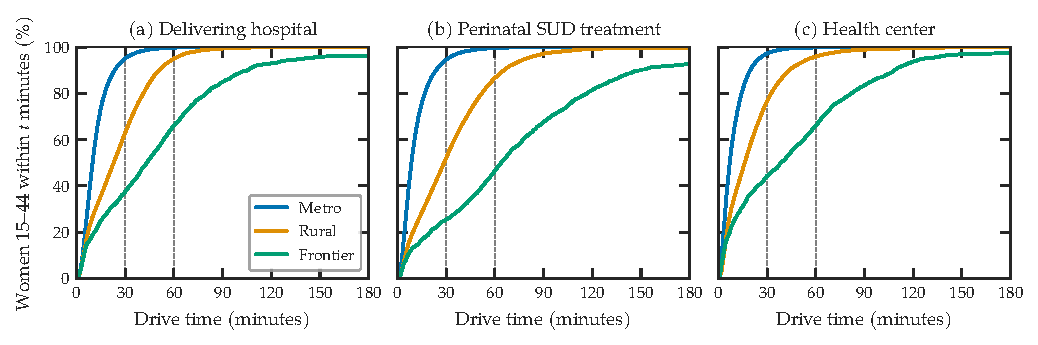
\includegraphics[width=\textwidth]{fig_coverage.pdf}
\caption{Share of women aged 15--44 living within $t$ minutes' drive of the nearest (a) delivering hospital, (b) perinatal SUD treatment facility, and (c) health center site, by county class (women-weighted cumulative distributions). Dashed lines mark 30 and 60 minutes. Curves that stay below 100\% at the right edge include women with no road route.}\label{fig:cov}
\end{figure*}

\begin{table*}[t]
\centering\small
\caption{Share of women aged 15--44 living more than 30 and more than 60 minutes' drive from the nearest site of each care type, by county class (percent). Women with no road route count as beyond. ``Upper bound'' adds hospitals whose labor and delivery status CMS does not report.}\label{tab:rur}
\begin{tabular}{@{}lrrrrrrrr@{}}
\toprule
 & \multicolumn{2}{c}{All} & \multicolumn{2}{c}{Metro} & \multicolumn{2}{c}{Rural} & \multicolumn{2}{c}{Frontier} \\
\cmidrule(lr){2-3} \cmidrule(lr){4-5} \cmidrule(lr){6-7} \cmidrule(lr){8-9}
Care type & $>$30 & $>$60 & $>$30 & $>$60 & $>$30 & $>$60 & $>$30 & $>$60 \\
\midrule
Delivering hospital (confirmed) & 9.0 & 1.0 & 4.9 & 0.2 & 37.0 & 5.0 & 62.6 & 34.1 \\
Delivering hospital (upper bound) & 7.4 & 0.5 & 4.3 & 0.1 & 29.3 & 2.3 & 41.1 & 15.8 \\
Obstetric clinician ZIP & 5.4 & 0.7 & 2.1 & 0.1 & 26.6 & 2.8 & 80.0 & 47.3 \\
Perinatal SUD treatment facility & 10.8 & 2.2 & 5.5 & 0.4 & 48.0 & 13.3 & 74.6 & 53.4 \\
Mental health facility (any) & 4.3 & 0.5 & 2.1 & 0.1 & 18.7 & 2.0 & 47.4 & 24.6 \\
Health center site & 5.5 & 0.8 & 2.8 & 0.1 & 23.4 & 4.1 & 55.7 & 33.9 \\
\midrule
Counties & \multicolumn{2}{c}{3{,}144} & \multicolumn{2}{c}{1{,}164} & \multicolumn{2}{c}{1{,}563} & \multicolumn{2}{c}{417} \\
Women 15--44 (thousands) & \multicolumn{2}{c}{65{,}971} & \multicolumn{2}{c}{57{,}923} & \multicolumn{2}{c}{7{,}624} & \multicolumn{2}{c}{423} \\
\bottomrule
\end{tabular}

\end{table*}

\begin{figure*}[t]
\centering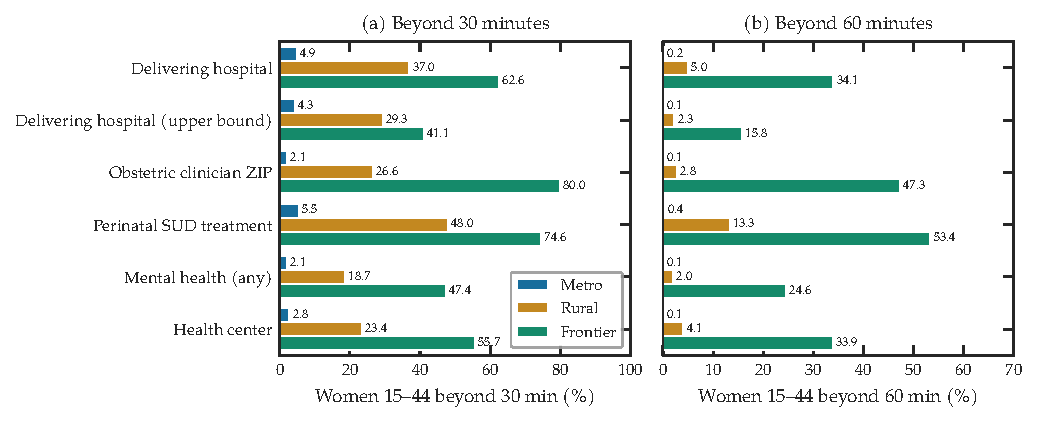
\includegraphics[width=\textwidth]{fig_bars.pdf}
\caption{Women aged 15--44 living more than (a) 30 and (b) 60 minutes from the nearest site of each of the six care types, by county class.}\label{fig:bars}
\end{figure*}

Figure~\ref{fig:bars} sets all six care types side by side. Two contrasts stand out. In rural counties, the share beyond 60 minutes is \PPWRuralSixty\% for perinatal SUD treatment against \OBRuralSixty\% for delivering hospitals and \HCRuralSixty\% for health centers, so perinatal SUD programs are about three times as far out of reach as the two general services. In frontier counties all three headline types leave a third or more of women beyond an hour.

\subsection{Geography}
Figure~\ref{fig:map} maps the county share of women beyond 60 minutes. Long drives to delivering hospitals concentrate in the Great Plains, the interior West, west Texas, Alaska, and pockets of the South and Appalachia. The perinatal SUD map is far darker: most of the northern and central Plains, much of Montana, Wyoming, Nevada, eastern Oregon, west Texas, and Alaska, and scattered counties across the South. Health center access (Fig.~\ref{fig:map2}a) is good in most of the South and East but poor across the Plains and interior West. By state (Fig.~\ref{fig:states}, Table~\ref{tab:states}), the largest shares of women beyond an hour from perinatal SUD treatment are in \TopStateOne\ (\TopStateOnePPW\%), \TopStateTwo\ (\TopStateTwoPPW\%), \TopStateThree\ (\TopStateThreePPW\%), \TopStateFour\ (\TopStateFourPPW\%), and \TopStateFive\ (\TopStateFivePPW\%); \StatesPPWOverTen\ states exceed 10\%.

\begin{figure*}[t]
\centering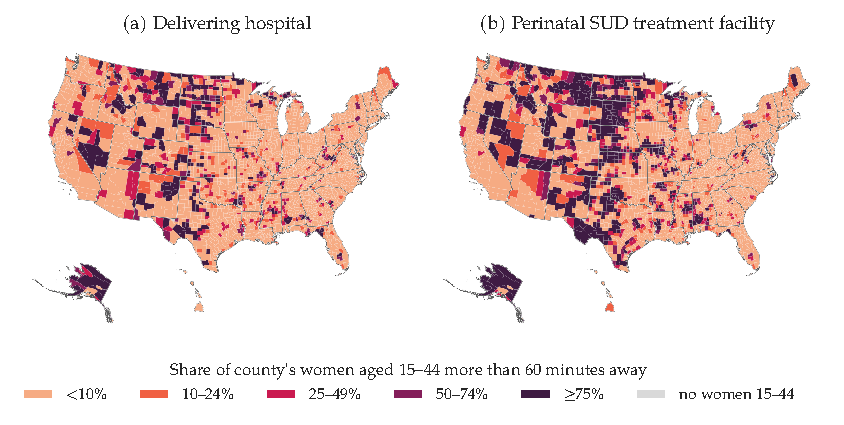
\includegraphics[width=\textwidth]{fig_map_ob_ppw.pdf}
\caption{Share of each county's women aged 15--44 living more than 60 minutes' drive from (a) a delivering hospital (confirmed list) and (b) a substance use treatment facility serving pregnant or postpartum women. Alaska (scaled) and Hawaii are shown as insets.}\label{fig:map}
\end{figure*}

\begin{figure*}[t]
\centering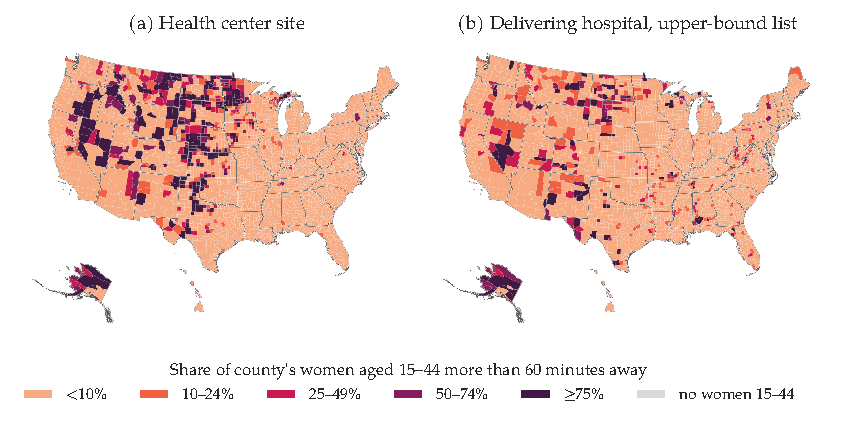
\includegraphics[width=\textwidth]{fig_map_hc_upper.pdf}
\caption{Share of each county's women aged 15--44 living more than 60 minutes' drive from (a) a HRSA health center site and (b) a delivering hospital on the upper-bound list. Panel (b) is the lower bound on hospital travel; compare with Fig.~\ref{fig:map}(a).}\label{fig:map2}
\end{figure*}

\begin{figure}[tbp]
\centering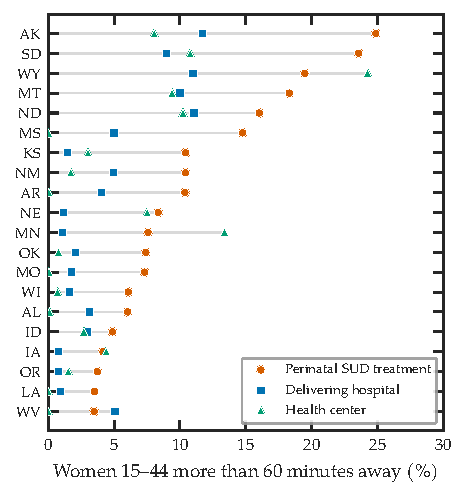
\includegraphics[width=\columnwidth]{fig_states.pdf}
\caption{The 20 states with the largest share of women aged 15--44 more than 60 minutes from a perinatal SUD treatment facility, with the corresponding shares for delivering hospitals and health centers.}\label{fig:states}
\end{figure}

\begin{table}[tbp]
\centering\footnotesize
\caption{The 12 states with the largest share of women aged 15--44 more than 60 minutes from perinatal SUD treatment (percent beyond 60 minutes).}\label{tab:states}
\begin{adjustbox}{max width=\columnwidth}\begin{tabular}{@{}lrrrr@{}}
\toprule
State & Women 15--44 & Hospital & PPW SUD & Health ctr. \\
\midrule
AK & 145{,}641 & 11.7 & 24.9 & 8.1 \\
SD & 167{,}665 & 9.0 & 23.6 & 10.8 \\
WY & 109{,}187 & 11.0 & 19.5 & 24.2 \\
MT & 207{,}746 & 10.0 & 18.3 & 9.4 \\
ND & 156{,}458 & 11.1 & 16.0 & 10.2 \\
MS & 584{,}757 & 5.0 & 14.8 & 0.0 \\
KS & 573{,}832 & 1.5 & 10.4 & 3.0 \\
NM & 405{,}272 & 4.9 & 10.4 & 1.7 \\
AR & 592{,}370 & 4.0 & 10.4 & 0.1 \\
NE & 386{,}076 & 1.1 & 8.3 & 7.5 \\
MN & 1{,}108{,}495 & 1.1 & 7.6 & 13.4 \\
OK & 802{,}035 & 2.1 & 7.4 & 0.8 \\
\bottomrule
\end{tabular}
\end{adjustbox}
\end{table}

\subsection{Counties cut off from care}
Table~\ref{tab:counties} counts counties in which most women live beyond each threshold, and Fig.~\ref{fig:cdist} shows the full distribution of county shares. In \MajSixtyPPW\ counties most women live more than an hour from perinatal SUD treatment (\MajSixtyPPWRural\ rural and \MajSixtyPPWFrontier\ frontier); in \AllSixtyPPW\ counties every woman does. The corresponding counts are \MajSixtyOB\ counties for delivering hospitals and \MajSixtyHC\ for health centers. In \RFMajSixtyPPWNotOB\ rural or frontier counties most women are more than an hour from perinatal SUD treatment while most are within an hour of a delivering hospital, where screening during prenatal and delivery care could occur but treatment referral would require long travel.

\begin{table}[tbp]
\centering\footnotesize
\caption{Counties in which more than half of women aged 15--44 live beyond 30 or 60 minutes, by care type and county class.}\label{tab:counties}
\begin{adjustbox}{max width=\columnwidth}\begin{tabular}{@{}lrrrrrr@{}}
\toprule
 & \multicolumn{3}{c}{Majority $>$30 min} & \multicolumn{3}{c}{Majority $>$60 min} \\
\cmidrule(lr){2-4}\cmidrule(lr){5-7}
Care type & Metro & Rural & Frontier & Metro & Rural & Frontier \\
\midrule
Delivering hospital (confirmed) & 275 & 790 & 345 & 5 & 110 & 190 \\
Delivering hospital (upper bound) & 210 & 520 & 209 & 2 & 35 & 88 \\
Obstetric clinician ZIP & 144 & 581 & 374 & 2 & 65 & 243 \\
Perinatal SUD treatment facility & 252 & 936 & 370 & 12 & 278 & 278 \\
Mental health facility (any) & 77 & 354 & 278 & 2 & 39 & 147 \\
Health center site & 110 & 416 & 294 & 6 & 88 & 181 \\
\midrule
Counties in group & 1{,}164 & 1{,}563 & 416 & 1{,}164 & 1{,}563 & 416 \\
\bottomrule
\end{tabular}
\end{adjustbox}
\end{table}

\begin{figure}[tbp]
\centering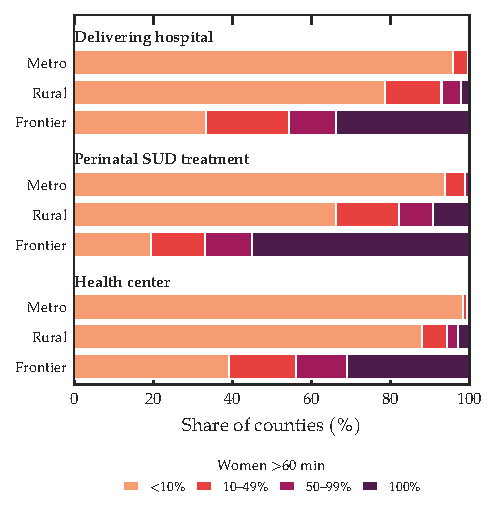
\includegraphics[width=\columnwidth]{fig_county_dist.pdf}
\caption{Distribution of counties by the share of their women aged 15--44 living more than 60 minutes from each headline care type, by county class.}\label{fig:cdist}
\end{figure}

\AllThree\ counties have most women more than an hour from all three headline care types. All are rural or frontier: \AllThreeFrontier\ are frontier and \AllThreeSmall\ have fewer than 500 women aged 15--44 (\AllThreeWomen\ women in all), spread across \AllThreeStates\ states, led by \AllThreeTopStates. These are mostly very small, sparsely settled counties whose shares rest on few people; half lie in Montana, the Dakotas, and Nebraska, where groups of adjacent counties have no type of perinatal care within an hour.

Across counties, median drive times to the three care types are moderately correlated (Spearman $\rho=\RhoOBPPW$ between delivering hospitals and perinatal SUD treatment, \RhoOBHC\ between hospitals and health centers, and \RhoPPWHC\ between perinatal SUD treatment and health centers; Fig.~\ref{fig:joint}). Many rural counties lie well above the diagonal in Fig.~\ref{fig:joint}: close to a delivering hospital, far from perinatal SUD treatment.

\begin{figure}[tbp]
\centering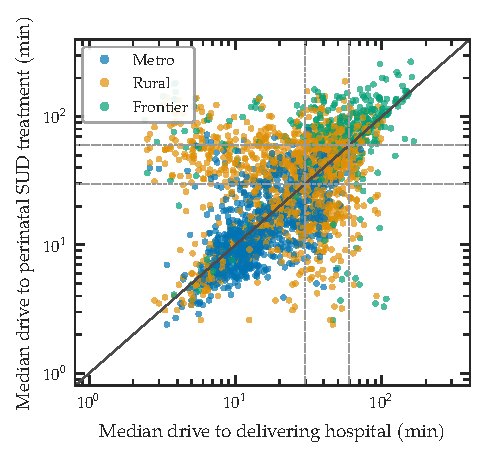
\includegraphics[width=\columnwidth]{fig_joint.pdf}
\caption{County women-weighted median drive to a delivering hospital against that to perinatal SUD treatment (log scales). Points above the diagonal are farther from perinatal SUD treatment than from a delivering hospital. Dashed lines mark 30 and 60 minutes.}\label{fig:joint}
\end{figure}

\subsection{County counts versus drive times}
Table~\ref{tab:xtab} compares the presence of a site inside a rural or frontier county with whether most of its women live within 30 minutes of one. The two views agree for \XPPWAgree\% of counties for perinatal SUD treatment, but disagree in both directions. Of the \XPPWNone\ rural or frontier counties with no perinatal SUD listing inside the county, \XPPWNoneReach\ have most women within 30 minutes of one across the county line; a county count would call them unserved. Conversely, \XPPWInFar\ counties with a listing inside still leave most women more than 30 minutes away; a count would call them served. The same pattern holds for delivering hospitals: \XOBNoneReach\ counties without a hospital are served from next door, and \XOBInFar\ counties with one leave most women more than 30 minutes away.

\begin{table}[tbp]
\centering\footnotesize
\caption{Rural and frontier counties by whether a site lies inside the county and whether most women live within 30 minutes of one.}\label{tab:xtab}
\begin{adjustbox}{max width=\columnwidth}\begin{tabular}{@{}llrr@{}}
\toprule
Care type & Site inside county? & Most women $\le$30 min & Most women $>$30 min \\
\midrule
Delivering hospital & Yes & 694 & 27 \\
 & No & 150 & 1{,}108 \\
Perinatal SUD facility & Yes & 557 & 38 \\
 & No & 116 & 1{,}268 \\
\bottomrule
\end{tabular}
\end{adjustbox}
\end{table}

\subsection{Sensitivity to the hospital list}
Adding the \SitesOBAdded\ hospitals whose labor and delivery status CMS does not report shortens the drive for \SensWomenChangeMillions\ million women and changes the picture most where it matters most (Fig.~\ref{fig:sens}, Fig.~\ref{fig:map2}b). The share of frontier women beyond 60 minutes falls from \OBFrontierSixty\% to \OBUFrontierSixty\%, the rural share from \OBRuralSixty\% to \OBURuralSixty\%, and the number of rural and frontier women beyond an hour from \RFWomenSixtyOB\ to \RFWomenSixtyOBU. In \SensCountiesChange\ counties the share beyond an hour drops by more than 25 percentage points. Because some of the added hospitals do deliver babies and some do not, the true rural and frontier values lie between the two lists; resolving these hospitals is the most valuable single improvement to the measure.

\begin{figure}[tbp]
\centering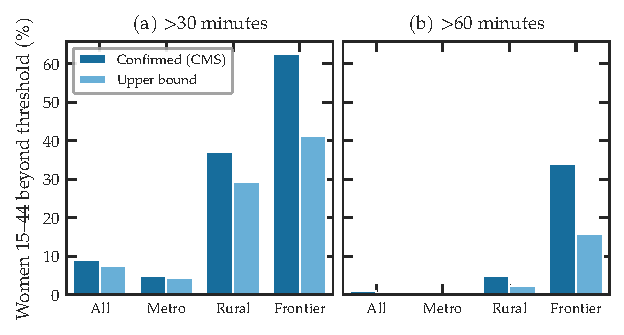
\includegraphics[width=\columnwidth]{fig_sensitivity.pdf}
\caption{Share of women aged 15--44 beyond (a) 30 and (b) 60 minutes from a delivering hospital under the confirmed and upper-bound hospital lists, by county class.}\label{fig:sens}
\end{figure}

\subsection{Agreement with OSRM and published estimates}
For the \ValN\ check trips, this study's times and OSRM's agree closely (Fig.~\ref{fig:val}, Table~\ref{tab:val}). The median ratio of times is \ValRatio, \ValWithin\% of trips agree within 20\% or 5 minutes, the mean absolute difference is \ValMAD\ minutes, and Pearson $r=\ValR$. The mean difference is \ValMeanDiff\ minutes with 95\% limits of agreement from \ValLoaLow\ to \ValLoaHigh\ minutes; 90\% of trips differ by less than \ValPNinetyAbs\ minutes and \ValNAbsTen\ by more than 10. Classification agrees for \ValAgreeThirty\% of trips at 30 minutes and \ValAgreeSixty\% at 60 minutes. Metro times run slightly faster (median ratio \ValRatioMetro) because OSRM adds turn and signal penalties; rural and frontier ratios are \ValRatioRural\ and \ValRatioFrontier. The largest differences occur in frontier block groups, where the two methods can attach the same origin to different roads.

\begin{figure*}[tb]
\centering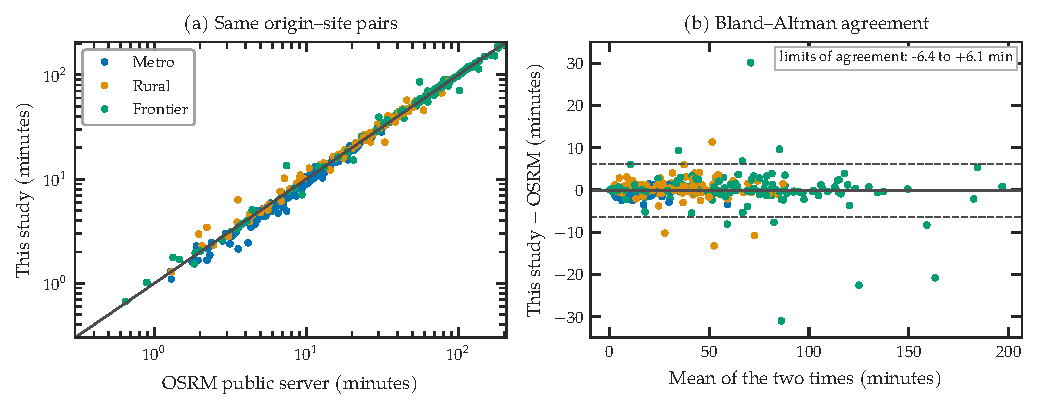
\includegraphics[width=0.92\textwidth]{fig_validation.pdf}
\caption{Drive times for the same \ValN\ origin--site pairs from this study and from the public OSRM server. (a) Times on log scales with the line of equality. (b) Bland--Altman plot of the difference against the mean; dashed lines are the 95\% limits of agreement.}\label{fig:val}
\end{figure*}

\begin{table}[tbp]
\centering\footnotesize
\caption{Agreement with the OSRM server by stratum. MAD: mean absolute difference.}\label{tab:val}
\begin{adjustbox}{max width=\columnwidth}\begin{tabular}{@{}lrrrrrr@{}}
\toprule
Stratum & $n$ & Median ratio & MAD (min) & $r$ & Agree 30 (\%) & Agree 60 (\%) \\
\midrule
All trips & 450 & 0.992 & 1.4 & 0.996 & 98.7 & 99.1 \\
\addlinespace
Metro & 150 & 0.940 & 0.8 & 0.996 & 98.7 & 99.3 \\
Rural & 150 & 1.003 & 1.2 & 0.993 & 98.7 & 99.3 \\
Frontier & 150 & 0.998 & 2.1 & 0.993 & 98.7 & 98.7 \\
\addlinespace
Delivering hospital & 150 & 0.992 & 1.5 & 0.991 & 98.7 & 98.0 \\
Perinatal SUD facility & 150 & 0.995 & 1.3 & 0.997 & 98.7 & 99.3 \\
Health center & 150 & 0.988 & 1.2 & 0.997 & 98.7 & 100.0 \\
\bottomrule
\end{tabular}
\end{adjustbox}
\end{table}

The national mean drive to a delivering hospital, \OBMeanNat\ minutes, matches the \FontenotMean\ minutes reported by Fontenot and colleagues from tract centroids on a commercial network~\cite{fontenot2024}. The share within 30 minutes (\OBWithinThirtyNat\%) is close to the \RayburnThirty\% reported by Rayburn and colleagues and the share within 60 minutes (\OBWithinSixtyNat\%) to their \RayburnSixty\%~\cite{rayburn2012}, although that study counted women aged 18--39 with 2007 hospital data and 2010 population, so the comparison is approximate.

\subsection{Nevada}
Table~\ref{tab:nv} shows the author's home state. Statewide, \NVOBSixty\% of Nevada's \NVWomen\ women aged 15--44 live more than an hour from a delivering hospital and \NVPPWSixty\% from perinatal SUD treatment, because most live in Clark and Washoe counties. The rural and frontier counties tell a different story. In \NVN\ counties (\NVList) no woman lives within an hour of a delivering hospital, and in \NVNPPW\ (\NVListPPW) none lives within an hour of perinatal SUD treatment. White Pine County is served by the Ely hospital but lies about three hours from the nearest perinatal SUD program, in Delta, Utah; Nye County's women live mostly in Pahrump, near treatment and a health center but about an hour from a delivering hospital in Las Vegas. These patterns agree with the author's earlier county mapping, which found seven Nevada counties without an OB/GYN provider and more than half without dedicated perinatal behavioral health services.

\begin{table}[tbp]
\centering\footnotesize
\caption{Nevada counties: women-weighted median drive (minutes) and share of women beyond 60 minutes for the headline care types. Hosp.: delivering hospital; PPW: perinatal SUD treatment; HC: health center.}\label{tab:nv}
\begin{adjustbox}{max width=\columnwidth}\begin{tabular}{@{}llrrrrrr@{}}
\toprule
 & & & \multicolumn{3}{c}{Median minutes} & \multicolumn{2}{c}{$>$60 min (\%)} \\
\cmidrule(lr){4-6}\cmidrule(lr){7-8}
County & Class & Women & Hosp. & PPW & HC & Hosp. & PPW \\
\midrule
Carson City & metro & 9{,}593 & 9 & 4 & 5 & 0 & 0 \\
Churchill & frontier & 4{,}484 & 11 & 9 & 70 & 0 & 0 \\
Clark & metro & 468{,}798 & 8 & 7 & 7 & 0 & 0 \\
Douglas & rural & 6{,}565 & 36 & 20 & 31 & 3 & 0 \\
Elko & frontier & 10{,}528 & 15 & 21 & 9 & 16 & 16 \\
Esmeralda & frontier & 131 & 147 & 146 & 146 & 100 & 100 \\
Eureka & frontier & 142 & 128 & 120 & 98 & 100 & 100 \\
Humboldt & frontier & 2{,}858 & 14 & 132 & 110 & 10 & 100 \\
Lander & frontier & 977 & 59 & 75 & 53 & 30 & 100 \\
Lincoln & frontier & 804 & 123 & 129 & 92 & 100 & 100 \\
Lyon & metro & 10{,}413 & 38 & 8 & 45 & 14 & 0 \\
Mineral & frontier & 733 & 90 & 71 & 141 & 100 & 94 \\
Nye & frontier & 6{,}893 & 67 & 10 & 11 & 86 & 13 \\
Pershing & frontier & 881 & 68 & 81 & 114 & 100 & 100 \\
Storey & metro & 442 & 40 & 28 & 14 & 0 & 0 \\
Washoe & metro & 97{,}840 & 10 & 9 & 7 & 0 & 0 \\
White Pine & frontier & 1{,}300 & 4 & 182 & 136 & 4 & 100 \\
\bottomrule
\end{tabular}
\end{adjustbox}
\end{table}

\FloatBarrier
\section{Discussion}\label{sec:disc}

\subsection{What the measures show}
Most women of reproductive age in the United States live within half an hour of a delivering hospital, a health center, and a perinatal SUD treatment program. The exceptions are concentrated where population is thin. In frontier counties a third of women live more than an hour from a delivering hospital or a health center and more than half from perinatal SUD treatment, and across the northern and central Plains whole groups of counties have no type of perinatal care within an hour. The most distinctive finding is the gap between obstetric and behavioral health access in rural counties: perinatal SUD programs are about three times as often out of reach as delivering hospitals. Because perinatal screening usually happens in obstetric settings, these are places where a positive screen can be obtained close to home but treatment designed for pregnant and postpartum women cannot.

\subsection{Implications for planning}
Three uses follow. First, the measures identify counties for service models that do not depend on travel: telehealth treatment and consultation, perinatal psychiatry access programs that support obstetric clinicians in managing behavioral health conditions~\cite{byatt2016}, mobile treatment, and co-location of SUD treatment with obstetric care in the hospitals and health centers that are close. Second, the comparison of county counts with drive times (Table~\ref{tab:xtab}) shows where count-based designations misclassify: counties without a program that are served from next door, and counties with a program that most of their women cannot reach. Third, because the method is open and runs on an ordinary computer, states can repeat it with their own facility lists, such as licensed birth centers, state-designated perinatal centers, or perinatal psychiatry programs, and with their own thresholds.

\subsection{Relation to previous work}
Our national hospital results agree with earlier commercial-network studies~\cite{rayburn2012,fontenot2024} despite different hospital lists and years, which supports the use of open roads and published routing speeds for this purpose. The decline documented by Ranchoff and colleagues~\cite{ranchoff2026} implies that the confirmed hospital measure should be refreshed as units close; the pipeline is designed for annual re-runs, each archived as a new version under the same concept DOI. To our knowledge this is the first national, county-level measure of travel time to SUD treatment programs for pregnant and postpartum women.

\subsection{Limitations}
The times are free-flow car times without traffic, weather, or seasonal closures; women without a car or who rely on public transportation face longer trips. Speeds follow standard routing-engine values rather than measured speeds, which leans conservative on rural highways (0.8 times a 55~mph limit is about 44~mph). The nearest site is not necessarily the one a woman uses, because insurance, level of care, waiting lists, language, and trust shape choices. CMS under-lists rural delivering hospitals, which the upper-bound list brackets, and freestanding birth centers are not included. The perinatal treatment flag covers substance use programs only; no open national list identifies perinatal mental health programs, and telehealth care is not counted. Neighborhood centers stand in for every home, which understates the spread of drive times within large frontier block groups. Places with no road route within 600 minutes, including islands without a car connection and Southeast Alaska towns served by the state ferry (whose long crossings exceed the limit at the default ferry speed), are reported as unreachable rather than given air, boat, or ferry times. Site coordinates are taken as published or geocoded, and errors within the correct state are not caught. The OSRM comparison checks the routing computation, not the completeness of the road map. Data years differ by source (Table~\ref{tab:sources}), and small counties' shares are unstable.

\section{Conclusions}\label{sec:concl}
We released an open, reproducible measure of drive-time access to delivering hospitals, perinatal SUD treatment, and health centers for every U.S.\ county, with rural and frontier results, an upper bound for under-reported hospitals, and a check against a standard routing engine. Access is good for most women but poor across the rural and frontier interior, and perinatal SUD treatment is the least accessible of the three services by a wide margin. Joined with the need and capacity measures of Project~1 on the shared county key, the release provides the travel layer for a public, national county map of perinatal behavioral health readiness.

\section*{Data and code availability}
Data, code, codebook, routing method notes, quality report, and provenance log: \url{https://github.com/memesobum/perinatal-access-layer}; archived on Zenodo, doi:\DOI. Licenses: code MIT; data and documents CC BY 4.0; road-derived values contain information from OpenStreetMap, \copyright\ OpenStreetMap contributors, available under the Open Database License.

\section*{Use of AI tools}
Claude (Anthropic) assisted with code and data handling. The author made every measurement decision and verified the results.

\section*{Competing interests and funding}
None declared. No funding was received.

\begin{thebibliography}{99}
\bibitem{cdc_mmrc2020} Centers for Disease Control and Prevention. Pregnancy-related deaths: data from maternal mortality review committees in 38 U.S. states, 2020. Atlanta, GA: CDC; 2024.
\bibitem{bauman2020} B.~L. Bauman, J.~Y. Ko, S.~Cox, et~al. Vital signs: postpartum depressive symptoms and provider discussions about perinatal depression---United States, 2018. \emph{MMWR Morb. Mortal. Wkly. Rep.}, 69(19):575--581, 2020. doi:10.15585/mmwr.mm6919a2
\bibitem{luca2020} D.~L. Luca, C.~Margiotta, C.~Staatz, et~al. Financial toll of untreated perinatal mood and anxiety disorders among 2017 births in the United States. \emph{Am. J. Public Health}, 110(6):888--896, 2020. doi:10.2105/AJPH.2020.305619
\bibitem{acog_cpg4} American College of Obstetricians and Gynecologists. Screening and diagnosis of mental health conditions during pregnancy and postpartum: Clinical Practice Guideline No.~4. \emph{Obstet. Gynecol.}, 141(6):1232--1261, 2023. doi:10.1097/AOG.0000000000005200
\bibitem{meinhofer2020} A.~Meinhofer, J.~M. Hinde, and M.~M. Ali. Substance use disorder treatment services for pregnant and postpartum women in residential and outpatient settings. \emph{J. Subst. Abuse Treat.}, 110:9--17, 2020. doi:10.1016/j.jsat.2019.12.005
\bibitem{patrick2020} S.~W. Patrick, M.~R. Richards, W.~D. Dupont, et~al. Association of pregnancy and insurance status with treatment access for opioid use disorder. \emph{JAMA Netw. Open}, 3(8):e2013456, 2020. doi:10.1001/jamanetworkopen.2020.13456
\bibitem{andrilla2018} C.~H.~A. Andrilla, D.~G. Patterson, L.~A. Garberson, et~al. Geographic variation in the supply of selected behavioral health providers. \emph{Am. J. Prev. Med.}, 54(6 Suppl 3):S199--S207, 2018. doi:10.1016/j.amepre.2018.01.004
\bibitem{hung2017} P.~Hung, C.~E. Henning-Smith, M.~M. Casey, and K.~B. Kozhimannil. Access to obstetric services in rural counties still declining, with 9 percent losing services, 2004--14. \emph{Health Aff.}, 36(9):1663--1671, 2017. doi:10.1377/hlthaff.2017.0338
\bibitem{kozhimannil2018} K.~B. Kozhimannil, P.~Hung, C.~Henning-Smith, M.~M. Casey, and S.~Prasad. Association between loss of hospital-based obstetric services and birth outcomes in rural counties in the United States. \emph{JAMA}, 319(12):1239--1247, 2018. doi:10.1001/jama.2018.1830
\bibitem{luo2003} W.~Luo and F.~Wang. Measures of spatial accessibility to health care in a GIS environment: synthesis and a case study in the Chicago region. \emph{Environ. Plann. B Plann. Des.}, 30(6):865--884, 2003. doi:10.1068/b29120
\bibitem{rayburn2012} W.~F. Rayburn, M.~E. Richards, and E.~C. Elwell. Drive times to hospitals with perinatal care in the United States. \emph{Obstet. Gynecol.}, 119(3):611--616, 2012. doi:10.1097/AOG.0b013e318242b4cb
\bibitem{fontenot2024} J.~Fontenot, C.~Brigance, R.~Lucas, and A.~Stoneburner. Navigating geographical disparities: access to obstetric hospitals in maternity care deserts and across the United States. \emph{BMC Pregnancy Childbirth}, 24:350, 2024. doi:10.1186/s12884-024-06535-7
\bibitem{ranchoff2026} B.~L. Ranchoff, A.~Kofner, O.~Baker, et~al. Obstetric service availability and travel time to access obstetric services in the U.S., 2010--2021. \emph{Am. J. Prev. Med.}, 71(2):108315, 2026. doi:10.1016/j.amepre.2026.108315
\bibitem{weiss2018} D.~J. Weiss, A.~Nelson, H.~S. Gibson, et~al. A global map of travel time to cities to assess inequalities in accessibility in 2015. \emph{Nature}, 553(7688):333--336, 2018. doi:10.1038/nature25181
\bibitem{weiss2020} D.~J. Weiss, A.~Nelson, C.~A. Vargas-Ruiz, et~al. Global maps of travel time to healthcare facilities. \emph{Nat. Med.}, 26(12):1835--1838, 2020. doi:10.1038/s41591-020-1059-1
\bibitem{emesobum_p1} M.~A. Emesobum. U.S. County Perinatal Behavioral Health Need and Capacity Panel (Version 0.1.0) [Data set]. Zenodo, 2026. doi:10.5281/zenodo.24025395
\bibitem{cenpop} U.S. Census Bureau. Centers of population by block group, 2020 Census. \url{https://www2.census.gov/geo/docs/reference/cenpop2020/}
\bibitem{haklay2008} M.~Haklay and P.~Weber. OpenStreetMap: user-generated street maps. \emph{IEEE Pervasive Comput.}, 7(4):12--18, 2008. doi:10.1109/MPRV.2008.80
\bibitem{luxen2011} D.~Luxen and C.~Vetter. Real-time routing with OpenStreetMap data. In \emph{Proc. 19th ACM SIGSPATIAL Int. Conf. Advances in Geographic Information Systems}, 513--516, 2011. doi:10.1145/2093973.2094062
\bibitem{dijkstra1959} E.~W. Dijkstra. A note on two problems in connexion with graphs. \emph{Numer. Math.}, 1:269--271, 1959. doi:10.1007/BF01386390
\bibitem{scipy2020} P.~Virtanen, R.~Gommers, T.~E. Oliphant, et~al. SciPy 1.0: fundamental algorithms for scientific computing in Python. \emph{Nat. Methods}, 17:261--272, 2020. doi:10.1038/s41592-019-0686-2
\bibitem{bland1986} J.~M. Bland and D.~G. Altman. Statistical methods for assessing agreement between two methods of clinical measurement. \emph{Lancet}, 327(8476):307--310, 1986. doi:10.1016/S0140-6736(86)90837-8
\bibitem{byatt2016} N.~Byatt, K.~Biebel, T.~A. Moore Simas, et~al. Improving perinatal depression care: the Massachusetts Child Psychiatry Access Project for Moms. \emph{Gen. Hosp. Psychiatry}, 40:12--17, 2016. doi:10.1016/j.genhosppsych.2016.03.002
\end{thebibliography}

\end{document}
